%                                                                 aa.dem
% AA vers. 8.2, LaTeX class for Astronomy & Astrophysics
% demonstration file
%                                                       (c) EDP Sciences
%-----------------------------------------------------------------------
%
%\documentclass[referee]{aa} % for a referee version
%\documentclass[onecolumn]{aa} % for a paper on 1 column  
%\documentclass[longauth]{aa} % for the long lists of affiliations 
%\documentclass[rnote]{aa} % for the research notes
%\documentclass[letter]{aa} % for the letters 
%\documentclass[authordate]{aa} % if the references are not structured 
% according to the author-year natbib style

%
\documentclass{aa}  

%\usepackage[author-year]{natbib}

%
\usepackage{graphicx}
%%%%%%%%%%%%%%%%%%%%%%%%%%%%%%%%%%%%%%%%
\usepackage{txfonts}
%%%%%%%%%%%%%%%%%%%%%%%%%%%%%%%%%%%%%%%%
%\usepackage[options]{hyperref}
% To add links in your PDF file, use the package "hyperref"
% with options according to your LaTeX or PDFLaTeX drivers.
%
\begin{document} 

   \title{Revisiting the $H_2$-$CO$ relationship in Taurus}
   \subtitle{}
   \author{K. Leschinski \inst{1}, A. Hacar\inst{1} \and J. Alves\inst{1}}
          

   \institute{Institute for Astronomy (IfA), University of Vienna,
              T\"urkenschanzstrasse 17, A-1180 Vienna\\
              \email{kdleschinski@gmail.com}
             }

   \date{Received -; accepted -}

\newcommand{\eco}{$C^{18}O$ }
\newcommand{\neco}{$N(C^{18}O)$ }
\newcommand{\ieco}{$I(C^{18}O)$ }
\newcommand{\av}{$A_V$ }
\newcommand{\htwo}{$H_2$ }
\newcommand{\nhtwo}{$N(H_2)$ }

% \abstract{}{}{}{}{} 
% 5 {} token are mandatory
  \abstract
  % context heading (optional)
  % {} leave it empty if necessary  
   {As the second most abundant molecule in the ISM, $CO$ plays a vital role in the star formation process. Hence accurate knowledge about its relationship to \htwo in the densest regions of the ISM is vital for accurately mapping \htwo in the regions where stars are born.}
  % aims heading (mandatory)
   {In this study we investigated the \eco -\htwo relationship along the 10pc-long L1495-B213 complex in Taurus. Aside from constraining the global \eco-\htwo relationship for the complex as a whole we investigated the extent to which this relationship varies on local (sub-parsec) scales.}
  % methods heading (mandatory)
   {To this end we generated extinction maps using the NICER method and the 2MASS catalogue. These maps were custom made to fit with the \eco integrated intensity map from \citet{hacar13}. The combined \eco-\av data-set was split into 7 sub-regions along extinction contours, roughly corresponding to those regions defined by \citet{barnard27}.}
  % results heading (mandatory)
   {We found a strongly linear relationship between \neco and \av for the range \av=[0$^m$, 20$^m$], with \neco $\propto 2.2\times 10^{14} A_V$ for the L1495-B213 complex as a whole. This agrres very well with the average value found in the literature, however it is 30\% greater than the value found by \citet{frerking82}. The gradient of the \neco-\av relationship differed by up to 20\% inside the 7 different sub-regions. The variation seen over the whole L1495-B213 complex covers the same range of variation reported in the literature (excluding \citealt{frerking82}) for several different molecular clouds.  We also found the minimum \htwo column density needed to shield \eco from the ISRF to be \nhtwo=$10^{21}$ cm$^{-2}$.}
  % conclusions heading (optional), leave it empty if necessary 
   {}
   \keywords{CO-AV Relationship, ISM, Molecular Hydrogen, Extinction}
   \maketitle


\section{Introduction}
Molecular Hydrogen is the most elusive of the fundamental building blocks of the universe. It forms in the coldest and densest regions of the galaxy, building large molecular clouds which are the birth places of stars. As such, an accurate knowledge of its distribution is of great importance for many aspects of astronomy. Unfortunately the homo-nuclear nature of the hydrogen molecule prevents the direct observation of the molecular gas at the temperatures (\~10K) found inside molecular clouds. Therefore the only way to map the distribution of \htwo is by the use of tracers. 

The relative ubiquity of dust in the interstellar medium (ISM) and its apparent constancy with relation to the hydrogen column density \citep{bohlin78} allows hydrogen column densities to be extrapolated from the measured dust column densities. However this includes the assumptions that there is a constant gas-to-dust ratio and, for determining \htwo column densities, that the vast majority of the intervening gas is in the form of molecular hydrogen \citet{bohlin78}. Furthermore, this method is limited by both the spatial density of background stars and the depth of the observations. Extinction maps for molecular clouds close to the galactic plane are therefore able to achieve much higher resolution than for those in the direction of the galactic poles. Fortunately, extinction methods are, however, unaffected by optical effects (line emission saturation) or chemical effects (photodissociation or "freezing-out") inside a molecular cloud. This makes this method useful for determining the total line of sight \htwo mass. In this study we used the NICER method\citep{nicer} to construct maps of the \htwo column density using the $N(H_2)-A_V$ relationship from \citet{bohlin78}.

A more direct measure of the \htwo column density can be found by using the next most abundance molecule in the ISM: $CO$. Since the discovery of $CO$ in the ISM by \citet{wilson70}, numerous authors have studied the connection between \htwo and the isotopologues of $CO$ (e.g. \citealt{dickman78}, \citealt{frerking82}, \citealt{duvert86}, \citealt{lada94}, \citealt{alves99}, \citealt{kainulainen06},\citealt{pineda10}). Invariably the results have shown that the emission from the most common isotopologues, $^{12}C^{16}O$ and $^{13}C^{16}O$ (henceforth $^{12}CO$ and $^{13}CO$), saturates at relatively low \htwo column densities (\av<5$^m$) (\citealt{frerking82}, \citealt{lada94}, \citealt{hayakawa01}, \citealt{pineda08}). This means that $^{12}CO$ and $^{13}CO$ are able to trace the distribution of \htwo in the sparse ($A_V<1^m$) and diffuse ($1^m<A_V<5^m$) ISM, however they are of limited use when tracing the densest ($5^m<A_V$) regions of molecular clouds. As the densest regions are where the preverbial party is happening, a less abundant, and thereby optically thinner, tracer is required.

Less abundant isotopologues, e.g. $^{12}C^{18}O$ (henceforth $C^{18}O$), saturate at much higher \htwo column densities and as such, show a linear correlation to \nhtwo over a much greater range of extinction values. The lower abundance does, however, mean that these molecules are unable to shield themselves from the UV component of the interstellar radiation field (ISRF) at low gas column densities \citep{vanDishoeck88}. Consequently large populations of these isotopologues do not survive in the diffuse ($A_V<1^m$) ISM. Furthermore, their lower abundance means that much longer observation times are required to detect their emission. For example, \citet{wilson94} estimate \eco to be approx 8x less abundant than $^{13}CO$ and the difference in emission strength is also on the same order of magnitude. However, compared to the saturated $^{13}CO$ emission, the \eco emission remains optically thin in regions along the L1495-B213 complex used in this study where $A_V>5^m$. It is because of this fact that \eco emission is often used to probe the high density (\av>5$^m$) regions of filaments and cores (\citealt{onishi96}, \citealt{kainulainen06}) .

While many studies have already investigated the \neco-\av relationship for several molecular clouds as a whole, there is very little agreement in the literature regarding the gradient of the \neco-\av curve. In this study we have looked at 7 sub-regions along the 10pc long L1495-B213 molecular cloud complex in Taurus in order to determine to what extent different molecular cloud environments play a role in the variation seen in the \eco-\av (\eco-\htwo) relationship.



\section{Data and Methods}

    \begin{figure*}
    \centering
    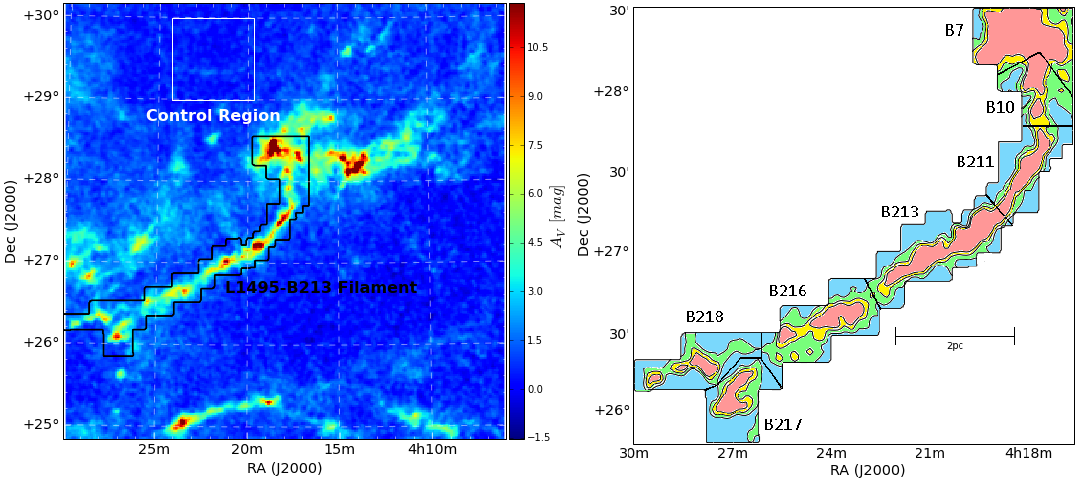
\includegraphics[width=\textwidth]{B-regions-horiz}
    \caption{(Left) The extinction map of the region of the Taurus molecular cloud complex used in this study. The black outline along the L1495-B213 complex shows the region covered by the $C^{18}O$ data set from \citet{hacar13}. The white box in the upper-left shows the region of low extinction used as a control field to determine the intrinsic stellar colours for this area of sky \citep{nicer}.  (Right) An illustration of the 7 sub-regions in L1495-B213. The contours shown are $A_V$=[$2.5^m$,$3.75^m$,$5^m$].}
    \label{Avmap}
    \end{figure*}

\subsection{\eco Data}
In this study we used the \eco ($J=1\to 0$) data published by \citet{hacar13} which covers 8 deg$^2$ along the L1495-B213 complex. The original observations have been re-convolved to have a FWHM beam size of 75'' and a grid spacing of 37.5''. \citet{hacar13} gives a full description of the observations and subsequent reduction process. For the purposes of this study we flattened the original data cube along the velocity axis in order to produce an integrated intensity map. According to \citet{hacar13} the rms pixel noise level in the $I($\eco$)$ data is 

[***GET UPDATED ERROR DATA***] 

$\sigma_I = 0.5\text{ K km s}^{-1}$, thus we discarded all data points in our analysis with integrated line intensities less than this threshold. The area covered corresponds to the dense regions of the L1495-B213 complex, where average extinction values are \av$>1^m$. Figure{fil6} shows the \av and \eco maps for the region of interest along the L1495-B213 complex.

We converted the integrated intensities, $I(C^{18}O)$, into line-of-sight column densities, $N(C^{18}O)$, by assuming a gas excitation temperature of $T_{ex}$=10K. This led to a conversion factor of $N(C^{18}O)/I(C^{18}O)=9.9 \times 10^{14}$. We maintain the assumption of a single excitation temperature is valid because a difference in the actual excitation temperature of $\pm3$K only introduces a maximum error of 5\% in the conversion factor. Thus even if $T_{ex}$ fluctuates between 7K and 13K, the measured column density will not vary wildly.

\subsection{\av data}

    \begin{figure}
    \centering
    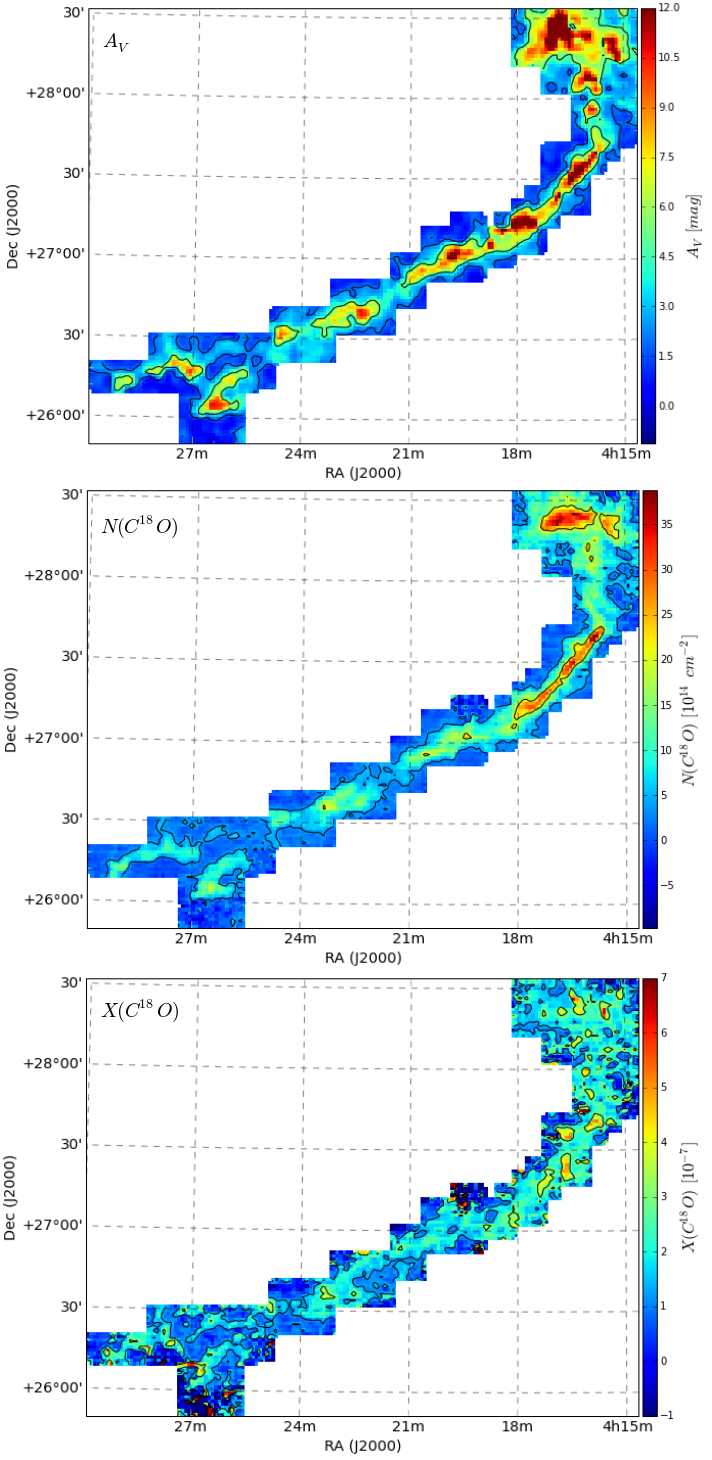
\includegraphics[width=0.45\textwidth]{Av_NCO_XCO}
    \caption{(Upper) The extinction map of the L1495-B213 complex used in this study. Contours are set to \av=[2$^m$,5$^m$]. (Middle) The map of \eco column density based on the integrated \eco intensities from \citet{hacar13} and assuming an excitation temperature of 10K. The contours are set to \neco=[4,20]$\times 10^{14}$ cm$^{-2}$. (Bottom) The map of \eco abundance with respect to \htwo - $X(C^{18}O/H_2)$. The contours are set to $X(C^{18}O/H_2)$=[1.33,3]$\times 10^{-7}$.}
    \label{fil6}
    \end{figure}

In order to study the relationship between \eco and \htwo we used the NICER method \citep{nicer} to generate extinction maps using the 2MASS point source catalogue (2MASS PSC). In order to avoid the inevitable introduction of uncertainties by converting between radio and tangential projections we generated individual extinction measurements for each pointing in the \eco integrated emission maps. This was done by reading in the central R.A and Dec. coordinates of each pixel in the \ieco map and extracting point sources from the 2MASS PSC \citep{2mass} located inside an aperture thrice the pixel-width around the pixel centre. The average extinction value for each star was calculated using the relationship from \citet{nicer}:

\begin{equation}
\hat{A}_V= \frac{C^{-1} \cdot \vec{k}}{\vec{k} \cdot C^{-1} \cdot \vec{k}}
\begin{pmatrix}
J-H - 0.49 \\ H-K_S - 0.13
\end{pmatrix}
\end{equation}

where k is the colour excess to extinction ratio given in \citet{rieke85} and is defined as $k_{ij}=E(i-j)/A_V$. For the case of J-H and H-K$_S$, we used $\vec{k}=(k_{J-H}, k_{H-K_S})=(0.107, 0.063)$. The factors 0.49 and 0.13 in equation 1 are the intrinsic average colours derived from the sample of stars in the control field (See Figure \ref{Avmap}). The inverse covariance matrix $C^{-1}$ is defined as the sum of the intrinsic variations in the colours J-H and H-K$_S$ and the individual magnitude uncertainties, $\sigma_i$:

\begin{equation}
C^{-1}=
\begin{pmatrix}
\sigma_{H^2}+\sigma_{K_S^2} + c_{22} & \sigma_{H^2} - c_{21} \\
\sigma_{H^2} - c_{12} & \sigma_{J^2}+\sigma_{H^2} + c_{11}
\end{pmatrix}
\end{equation}

with the coefficients $c_{ij}$ referring to the intrinsic scatter in the J-H and H-K$_S$ colours in the control field and $\sigma_{X^2}$ referring to the photometric uncertainty in the star's magnitude. See \citet{nicer} for a detailed description of the method. It should be noted that the covariance matrix must be recalculated for each source in the catalogue.

[***LOOK UP THE SQAURED SIGMAS AGAIN***]

The extinction map was generated to perfectly match the \ieco map and as such has a beam FWHM of 75" and spacing of 37.5". The minimum amount of stars used for each pixels extinction value was four. The corresponding average uncertainty was found to be $\sigma_{A_V} = 0.17^m$ for regions with $A_V<2^m$. The largest absolute uncertainty was $0.43^m$ for a line of sight with $A_V=18^m$.

The conversion from \av to \htwo was made using the standard conversion factor of $9.4 \times 10^20$, as derived from \citet{bohlin78} under the assumption of a standard reddening law ($A_V/E(B-V)=3.1$). It was also assumed that fraction of atomic hydrogen was negligible compared to the fraction of \htwo.

In order to check the consistency of our implementation of the NICER method, we compared our \av map to that of \citet{lombardi10}. The result was a mostly one-to-one correlation. We attributed the small variations at low extinctions to the re-projection of the two maps onto a common grid. The scatter seen at higher extinctions was attributed to the different methods used for determining the \av values (NICER (this study) vs NICEST \citep{lombardi10} - a comparison of these two techniques is given in \citealt{lombardi09}. The variation due to these factors, however, was not fatal to the outcomes of this study.


\subsection{Regions of Interest}
The \eco and \av data sets used in this study were each comprised of >14600 independent measurements. We investigated the relationship between \av and \eco for two scales: over the whole 10 pc long L1495-B213 complex to find a ''global'' \neco-\av relationship, and inside 7 sub-regions ($\sim$ 1 pc) to find the ''local'' relationship. Due to the shear volume of data we split up the L1495-B213 complex into the 7 sub-regions in order to investigate any possible spatial variation in the \eco-\av relationship. According to \citet{???}

[***check reference*** - possibly hacar13+]

the L1495-B213 complex is not evolving in a homogeneous manner. For example, \citet{rebull10} report a cluster of YSOs in the B7 sub-region, which indicates that certain parts of the cloud have already collapsed. The opposite is true of the adjacent B211 sub-region where only a single dense cores is seen. Hence we found it prudent to investigate the \av-\eco relationship separately for the different environments along the complex.

The division of the L1495-B213 complex was based on the extinction contours (See Figure \ref{Avmap}). The position of the borders between the sub-regions corresponded roughly to the those defined originally by \citet{barnard27} and more recently by \citet{schmalzl10}. Hence each region will be referred to by its Barnard catalogue reference: B7, B10, B211, B213, B216, B217 and B218. The $A_V=2.5^m$ contour was used to differentiate between the B216, B217 and B218 sub-regions. B216 and B213 were divided by the $A_V=3.75^m$ contour and the B10/B211 border is defined by the $A_V=5^m$ contour. The regions B7/B10 and B211/B213 were indistinguishable in extinction and so the cuts were defined by those used in \citet{schmalzl10} and \citet{hacar13} respectively. Each sub-region, except for B10, contained at least 1800 \eco and \av measurements. B10, with 1155 data points, still contained a statistically significant sample.


\section{Results and Discussion}

\subsection{The global relationship between \eco and \av}

    \begin{figure*}
    \centering
    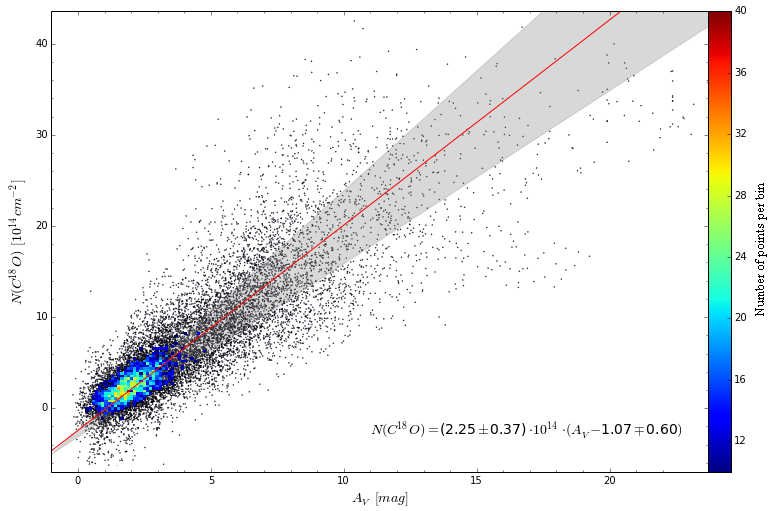
\includegraphics[width=\textwidth]{NCO_AV}
    \caption{The global relationship between \neco and \av for the L1495-B213 complex. The broad grey region represents the area between the linear least-squares fits applied to the data along each axis. The solid red line is the average of these best-fits. The nominal uncertainty in the \neco measurements is     [***fill in error***].     The uncertainty in the extinction measurements averaged 7\% and never exceed 20\% for areas where $A_V>2^m$. Errorbars have been omitted in this figure in order to better display the $\approx$ 14600 data points. The colourful region shows the density of points in bins of size ($d$\av, $d$\neco)=($0.1^m$, $0.2\times 10^14$ cm$^{-2}$).}
    \label{C18Oglobal}
    \end{figure*}

For each line-of-sight measurement of \neco along the L1495-B213 complex we determined an average extinction value. Figure \ref{C18Oglobal} shows a linear relationship between these two quantities for the whole range of extinctions probed ($A_V=[0^m, 20^m]$). A least-squares fit to the \neco-\av data reveals the relationship to be:

\begin{equation}
N(C^{18}O)=(2.25 \pm 0.37) \cdot 10^{14} \cdot (A_V - 1.07 \mp 0.60)
\end{equation}

where $N(C^{18}O)$ is the line of sight column density of $C^{18}O$ and has units of particles/cm$^2$. Extinction, \av, has units of magnitudes. The broad grey region in Figure \ref{C18Oglobal} represents the spread in the least-squares fit when fitting to a reversed set of axes. The lower boundary of the grey region represents the least-squares fit to data following the \av-axis, while the upper boundary represents the least-squares fit to the data along the \neco-axis.

[*** Try fitting the Gaussian to the spread - comment***]

It is clear from Figure \ref{C18Oglobal} that the \eco emission does not saturate within the range of extinction probed. This linearity in the relationship shows that \neco is a reliable tracer of the dust, and hence \htwo, for moderate extinctions ($2^m<A_V<20^m$) and possibly higher. This is in stark contrast to the emission from $^{13}CO$ which is only useful for tracing \htwo up to around $A_V \approx 5^m$ \citep{pineda08}. This therefore makes $^{13}CO$ useless for tracing the distribution of \htwo in the densest ($A_V>5^m$) regions of the ISM.

Another feature that is visible in Figure \ref{C18Oglobal} is the density of gas required to shield \eco molecules from the interstellar radiation field. We find this to be $A_{V,0}=1.07 \pm 0.6$ or a \htwo column density of \nhtwo=$(1.0 \pm 0..56) \times 10^21$. This compares favourably to the values found by \citet{frerking82}, \citet{duvert86} for observations in Taurus and with the models of \citet{vanDishoeck88}.

As expected with a sample of >14000 points there is large scatter present in Figure \ref{C18Oglobal}, however these outliers are somewhat distracting. The coloured region in Figure \ref{C18Oglobal} show where the regions of highest point density are. The vast majority of points are clustered around the line of best fit. The nominal total uncertainty in the individual measurements over the data set was calculated to be 20\% (extinction plus integrated line intensity) and is dominated by uncertainties in the extinction measurements.

[***Mention the gaussian again***]

By assuming a relative isotopologue ratio of 560 for $^{12}CO$ to \eco \citep{wilson94} and \nhtwo/\av=$9.4\times 10^{20}$ \citep{bohlin78} it is possible to estimate the $^{12}CO$-\htwo ratio for the L1495-B213 complex. We find this to be 

\begin{equation}
X(^{12}CO/H_2)=(1.34 \pm 0.22) \times 10^{-4}
\end{equation}

This value agrees, within the uncertainties, with the value found by \citet{pineda10} using $^{13}CO$ data. This value is 50\% higher than that found by \citet{frerking82}, however. As will be mentioned in Section 3.3, we assert that \citet{frerking82} underestimated the \eco-\htwo relationship in Taurus by $\sim$30\%. We have avoided making an estimate for the required minimum gas column density, $A_{V,0}$, because this is highly dependent on the local UV radiation field.


\subsection{Differences in observed C18O-Av ratios}

    \begin{figure*}
    \centering
    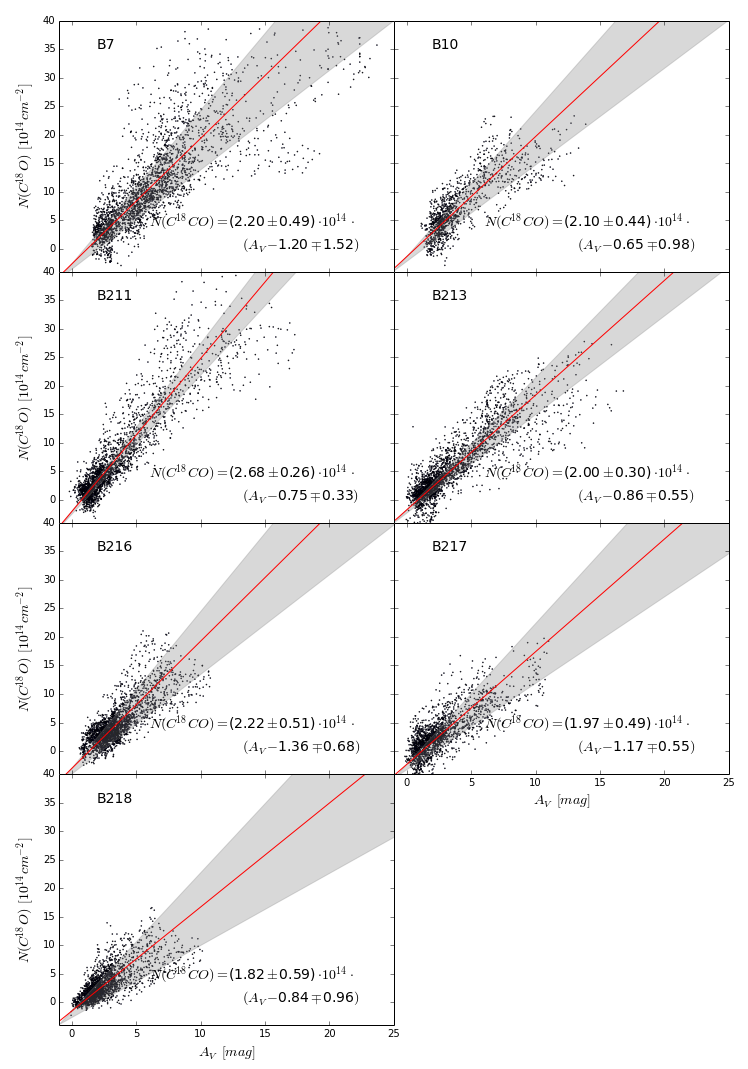
\includegraphics[width=0.85\textwidth]{N(C18O)_vs_AV_Bregions}
    \caption{The \neco-\av relationship for each of the sub-regions in the L1495-B213 complex. The average uncertainty in the \eco column density is 3\% while the nominal uncertainty for the extinction measurements is 17\%. Even though the scatter appears to be large it should be noted that in each sub-region between 66\% and 83\% of the data points lie within the solid black cloud located along the line of best-fit. It is clear that the B7 region is the main contributor to the noise seen in the global relationship. In general, the \neco-\av relationship in linear in all sub-regions and shows no signs of saturation with in the range of extinction probed.}
    \label{C18O_local}
    \end{figure*}

The size of the sample meant that it was possible to investigate the \neco-\av relationship on scales smaller than the L1495-B213 complex. Figure \ref{C18O_local} shows the \neco-\av relationship for each of the 7 sub-regions along with a linear least-squares fit to the data. The grey regions in Figure \ref{C18O_local} represent the difference in the best-fit curve when switching the axes. Table \ref{sub_region_pars} lists the parameters of the \neco -\av relationships for each of the sub-regions. Generally, the scatter seen in these sub-regions is much less than that seen in Figure \ref{C18Oglobal} for the whole L1495-B213 complex.

\begin{table}
\centering
\begin{tabular}{l|r|r}
Region & Gradient $m$ ($\sigma_m$) & $A_{V,0}$ ($\sigma_{Av,0)}$) \\
\hline
B7 & 2.20 (0.49) & 1.20 (1.52) \\
B10 & 2.10 (0.44) & 0.65 (0.98) \\
B211 & 2.68 (0.26) & 0.75 (0.33) \\
B213 & 2.00 (0.30) & 0.86 (0.55) \\
B216 & 2.22 (0.51) & 1.36 (0.68) \\
B217 & 1.97 (0.49) & 1.17 (0.55) \\
B218 & 1.82 (0.59) & 0.84 (0.96) \\
\hline
Global & 2.25 (0.37) & 1.07 (0.60)\\

\end{tabular}
\caption{Parameters for the least-squares fit to the relationship $$N(C^{18}O)\text{ [$10 ^{14}$ cm$^{-2}$]}=m\times (A_V - A_{V,0})$$ for each of the sub-regions. Here $A_{V,0}$ is seen as the \htwo column density required to shield the \eco population from the ISRF.}
\label{sub_region_pars}
\end{table}

There are very few surprises when comparing the parameters of the local \neco-\av relationships to the global relationship. The B7 region is responsible for the majority of the scatter seen in the Figure \ref{C18Oglobal}. The presence of a large number of YSOs in this region \citep{rebull10} is quite obviously disturbing the chemical equilibrium of the gas. Even so, the \neco-\av relationship is very close to that found for the L1495-B213 complex as a whole. There also appears to be two branches in the data - one extending towards higher extinctions and one extending towards high \eco column densities. The low \neco-high \av branch corresponds spatially to the region where many of the YSOs are located \citep{hacar13}. The other branch (high \neco, low \av) corresponds to the region directly west of the YSO cluster where the cloud has not yet started to collapse, or is being hindered by the increased ambient radiation from the YSOs. \citet{hacar13} also reports that the region does not yet contain any dense cores\footnote{This assertion is based on the lack of $N_2H^+$ emission, a tracer of the very dense gas ($A_V>20^m$)}.

The quiescent nature of the B211 sub-region, as inferred by its lack of dense cores or YSOs \citep{hacar13}, is reflected in the tightly correlated \neco-\av relationship. B211 also exhibits the highest ratio of \neco to \nhtwo of anywhere in the L1495-B213 complex.

[***insert reason why the quiet un-evolved gas should have a higher ratio***]

B218 exhibits the lowest gradient for the \neco-\av relationship. It also contains the least dense ($A_V>5^m$) gas. It may be argued that the abundance of diffuse gas and consequent destruction of \eco molecules by the interstellar radiation field is the reason for the weak \neco-\av ratio in B218.

The remaining regions - B10, B213, B216 and B217 all show a linear relationship between \neco and \av and have gradients similar to the global gradient. The interstellar radiation field (ISRF)-shielding value, $A_{V,0}$, for the survival of \eco molecules for these regions centres around $A_{V,0}=1^m$. This agrees well with the global ISRF-shielding value for the L1495-B213 complex as a whole. The mean \neco-\av relationship throughout these 7 sub-regions differs somewhat from the previously calculated global relationship\footnote{This difference to the global relationship may be attributed to the fact that regions with a greater mass of dense gas ($A_V>5^m$) i.e. B7, B211 and to some extent B213, had a greater influence on determining the best fit to the data at higher extinctions. These regions were also spatially the largest and therefore carried more weight in the fitting process.}:

\begin{equation}
N(C^{18}O) \text{ [cm$^{-2}$]}=(2.14 \pm 0.59) \cdot 10^{14} \cdot (A_V - 0.98 \mp 2.30)
\end{equation}

While it may be postulated that the difference in the \neco-\av relationship between sub-regions may be due to the amount of YSOs and dense cores in each one, a brief comparison using table 1 from \citet{hacar13}) showed no correlation.


\subsection{Comparison to the Literature}

    \begin{figure}
    \centering
    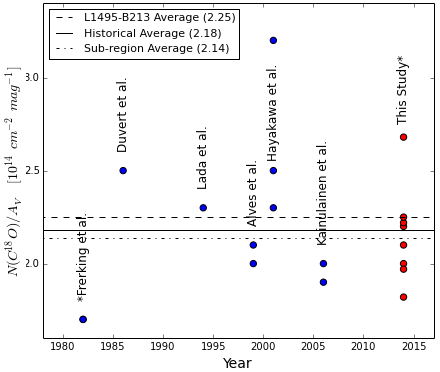
\includegraphics[width=0.5\textwidth]{History_dot_plot}
    \caption{A comparison between the gradient for the \eco-\av relationship found for each one the sub-regions in the L1495-B213 complex and 6 other studies conducted over the past 30 years.}
    \label
    {hist_dot_plot}
    \end{figure}

\citet{frerking82} were amongst the first to study the \neco-\av relationship in Taurus and, with over 700 citations, their paper has become a standard reference paper for the relationship between \htwo and $CO$. In the intervening 30 years the amount of data available for study has drastically increased and so too has our understanding of this relationship. Therefore we found it prudent to compare our results with those of \citet{frerking82}. Figure {frerkingme} shows this comparison. While the scatter described by \cite{frerking82} is still visible in our data, we are able to better quantify these outliers. We no longer see a discontinuity in the \neco-\av relationship at $A_V=4^m$ and we have much more complete data for extinctions greater than $A_V=10^m$. Ultimately we see that the equation given by \citet{frerking82} underestimates the \neco-\av relationship in Taurus by approximately 30\%\footnote{It should be noted that the \av values used by \citet{frerking82} were based on spectra towards single stars. We applied the NICER method to the pointings used by \citet{frerking82} and found agreement (within a range of $\pm$ 30\%) between the two methods for $A_V<10^m$. The two highest \av data points in \citet{frerking82} were out by a factor of 170\% and 260\% respectively. It should also be stated that \citet{frerking82} observed sources across a larger region of the Taurus molecular cloud complex than seen in this study. Their study includes sources from Heiles' Cloud 2, L1521 and B18 as well as from the L1495-B2213 complex.}.

Furthermore, we compared our results to six other studies of the \neco-\av relationship in other clouds (\citealt{frerking82}, \citealt{duvert86}, \citealt{lada94}, \citealt{alves99}, \citealt{hayakawa01}, \citealt{kainulainen06}). Figure \ref{hist_dot_plot} shows how the large differences in the gradient of the \neco-\av relationship between the individual studies are covered by the range of gradients seen in the sub-regions of the L1495-B213 complex. This suggests that while both the extra- and intra-cloud environments play a role in determining the strength of the local relationship between \neco and \av, there is a universal relationship underpinning the interaction between \neco and \htwo in all molecular clouds. 

    \begin{figure}
    \centering
    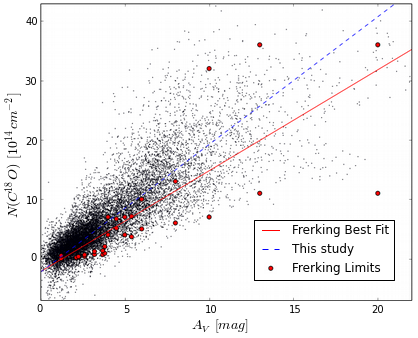
\includegraphics[width=0.5\textwidth]{mefrerking}
    \caption{A comparison between the whole data set used in this study and that used by \citet{frerking82}. The circles represent the upper and lower limits used by \citet{frerking82} for the \neco measurements and the solid line is the least-squares fit to these points. We see that the \neco values presented by \citet{frerking82} underestimate the true column density to varying degrees.}
    \label
    {mefrerking}
    \end{figure}

\section{Summary and Conclusions}

In this study we used the \eco data from \citet{hacar13} alongside custom-made extinction maps using the 2MASS PSC to determine the \eco-\htwo relatioship in 7 subregions of the L1495-B213 molecular cloud complex. Our main findings are as follows:

1. The gradient of the global \neco-\av relationship for the L1495-B213 complex was found to be \neco/\av~$=(2.25\pm0.37) \times 10^{14}$~cm$-2$. This value is  30\% greater than the value found by \citet{frerking82} for the Taurus cloud complex and 10\% less than that found by \citet{duvert86} for L1495. It was also within 4\% of the average gradient found in the literature for the \neco-\av relationship. 

2. The \neco-\av relationship was found to vary by $\pm$20\% throughout the 7 sub-regions of the L145-B213 complex.  All sub-regions exhibited a linear trend, proving that the \eco emission throughout the L1495-B213 complex is optically thin. The highest gradient was found in the quiescent region B211, while the wildest variations were found in the B7 region - a region known for its large population of YSOs. While tempting, no correlation was found between the number of YSOs and dense clumps and the variation in the \neco-\av relationship in each sub-region.

3. This variation seen in the 7 sub-regions of the L1495-B213 complex covers the range of variations seen in the literature. This shows that these variations are an intrinsic characteristic of the \neco-\av relationship and are not dependent on any cloud in particular. We also found that the oft-cited paper by \citet{frerking82} underestimates the \neco-\av relationship by 30\%.

4. We found the \htwo column density needed for \eco to be adequately shielded from the ISRF in the L1495-B213 complex was $N(H_2)=1.0 \times 10^{21}$ cm$-2$. This is consistent with other studies of regions without strong UV sources.

5. By assuming the $^{12}CO-C^{18}O$ abundance ratio of 560 \citep{wilson94} we extrapolated the global \neco-\av relationship to find the $^{12}CO$-\htwo ratio: $X(^{12}CO/H_2)=(1 .3\pm0.2)\times10^{-4}$. This value is consistent with that found in the literature using the more abundant isotopologues of $^{12}CO$ and $^{13}CO$. 


\section{Appendix - NICER}   
[Give and explanation of the covariance matrices in the NICER method here. - Is this needed?]


%______________________________________________________________


\begin{acknowledgements}
The author greatly acknowledges Dr. Alvaro Hacar for the constant guidance and insightful discussions during the course of this project. The author would also like to thank Dr. Joao Alves for the motivation to publish this work. This study took advantage of data from the Two Micron All Sky Survey (2MASS - \citealt{2mass}). The analysis of the data was conducted with the help of Topcat \citep{topcat} and Astropy \citep{astropy}.
\end{acknowledgements}


%-------------------------------------------------------------------

\begin{thebibliography}{}

\bibitem[Alves et al.(1999)]{alves99} Alves, J., Lada, C.~J., \& Lada, E.~A.\ 1999, \apj, 515, 265 

\bibitem[Astropy Collaboration et al.(2013)]{astropy} Astropy Collaboration, Robitaille, T.~P., Tollerud, E.~J., et al.\ 2013, \aap, 558, A33 

\bibitem[Barnard et al.(1927)]{barnard27} Barnard, E.~E., Frost, E.~B., \& Calvert, M.~R.\ 1927, [Washington] Carnegie institution of Washington, 1927., 

\bibitem[Bohlin et al. (1978)]{bohlin78} Bohlin, R.~C., Savage, B.~D., \& Drake, J.~F.\ 1978, \apj, 224, 132 

\bibitem[Bok (1937)]{bok37} Bok, B.~J.\ 1937, Chicago: University of Chicago Press, 1937

\bibitem[Dickman(1978)]{dickman78} Dickman, R.~L.\ 1978, \apjs, 37, 407 

\bibitem[Duvert et al.(1986)]{duvert86} Duvert, G., Cernicharo, J., \& Baudry, A.\ 1986, \aap, 164, 349 

\bibitem[Frerking et al.(1982)]{frerking82} Frerking, M.~A., Langer, W.~D., \& Wilson, R.~W.\ 1982, \apj, 262, 590 

\bibitem[Goldsmith et al.(2008)]{goldsmith08} Goldsmith, P.~F., Heyer, M., Narayanan, G., et al.\ 2008, \apj, 680, 428 

\bibitem[Hacar et al.(2013)]{hacar13} Hacar, A., Tafalla, M., Kauffmann, J., \& Kov{\'a}cs, A.\ 2013, \aap, 554, A55 

\bibitem[Hayakawa et al.(2001)]{hayakawa01} Hayakawa, T., Cambr{\'e}sy, L., Onishi, T., Mizuno, A., \& Fukui, Y.\ 2001, \pasj, 53, 1109 

\bibitem[Kainulainen et al.(2006)]{kainulainen06} Kainulainen, J., Lehtinen, K., \& Harju, J.\ 2006, \aap, 447, 597 

\bibitem[Lada et al.(1994)]{lada94} Lada, C.~J., Lada, E.~A., Clemens, D.~P., \& Bally, J.\ 1994, \apj, 429, 694 

\bibitem[Lombardi \& Alves(2001)]{nicer} Lombardi, M., \& Alves, J.\ 2001, \aap, 377, 1023 

\bibitem[Lombardi(2009)]{lombardi09} Lombardi, M.\ 2009, \aap, 493, 735 

\bibitem[Lombardi et al.(2010)]{lombardi10} Lombardi, M., Lada, C.~J., \& Alves, J.\ 2010, \aap, 512, A67 

\bibitem[Onishi et al.(1996)]{onishi96} Onishi, T., Mizuno, A., Kawamura, A., Ogawa, H., \& Fukui, Y.\ 1996, \apj, 465, 815 

\bibitem[Pineda et al.(2008)]{pineda08} Pineda, J.~E., Caselli, P., \& Goodman, A.~A.\ 2008, \apj, 679, 481 

\bibitem[Pineda et al.(2010)]{pineda10} Pineda, J.~L., Goldsmith, P.~F., Chapman, N., et al.\ 2010, \apj, 721, 686 

\bibitem[Planck Collaboration et al.(2011)]{planck11} Planck Collaboration, Ade, P.~A.~R., Aghanim, N., et al.\ 2011, \aap, 536, A19 

\bibitem[Rebull et al.(2010)]{rebull10} Rebull, L.~M., Padgett, D.~L., McCabe, C.-E., et al.\ 2010, \apjs, 186, 259 

\bibitem[Rieke \& Lebofsky(1985)]{rieke85} Rieke, G.~H., \& Lebofsky, M.~J.\ 1985, \apj, 288, 618 

\bibitem[Schlegel et al.(1998)]{schlegel98} Schlegel, D.~J., Finkbeiner, D.~P., \& Davis, M.\ 1998, \apj, 500, 525 

\bibitem[Skrutskie et al.(2006)]{2mass} Skrutskie, M.~F., Cutri, R.~M., Stiening, R., et al.\ 2006, \aj, 131, 1163 

\bibitem[Schmalzl et al.(2010)]{schmalzl10} Schmalzl, M., Kainulainen, J., Quanz, S.~P., et al.\ 2010, \apj, 725, 1327 


\bibitem[Taylor(2005)]{topcat} Taylor, M.~B.\ 2005, Astronomical Data Analysis Software and Systems XIV, 347, 29 

\bibitem[van Dishoeck \& Black(1988)]{vanDishoeck88} van Dishoeck, E.~F., \& Black, J.~H.\ 1988, \apj, 334, 771 

\bibitem[Wilson et al.(1970)]{wilson70} Wilson, R.~W., Jefferts, K.~B., \& Penzias, A.~A.\ 1970, \apjl, 161, L43 

\bibitem[Wilson \& Rood(1994)]{wilson94} Wilson, T.~L., \& Rood, R.\ 1994, \araa, 32, 191 

\end{thebibliography}

\end{document}